% Section: Results (manuscript agent owns prose and numbers).
% The tail-ledger table/figure below are generated from committed provenance
% files by scripts/make_release_tables.py and scripts/make_release_figures.py.
\subsection{Deep-tail ledger}
\begin{table}
  \centering
  \caption{Matched 3000-outer-period deep-tail ledger by reintegration chunk (seed 42).}
  \label{tab:tail_ledger}
  \begin{tabular}{lrrr}
    \toprule
    Outcome & Chunk 0 & Chunk 1 & Merged \\
    \midrule
    ejected & 20,064 & 20,015 & 40,079 \\
    stable & 29,905 & 29,948 & 59,853 \\
    numerical\_error & 31 & 36 & 67 \\
    collision & 0 & 1 & 1 \\
    \midrule
    Total & 50,000 & 50,000 & 100,000 \\
    \bottomrule
  \end{tabular}
\end{table}


\begin{figure}
  \centering
  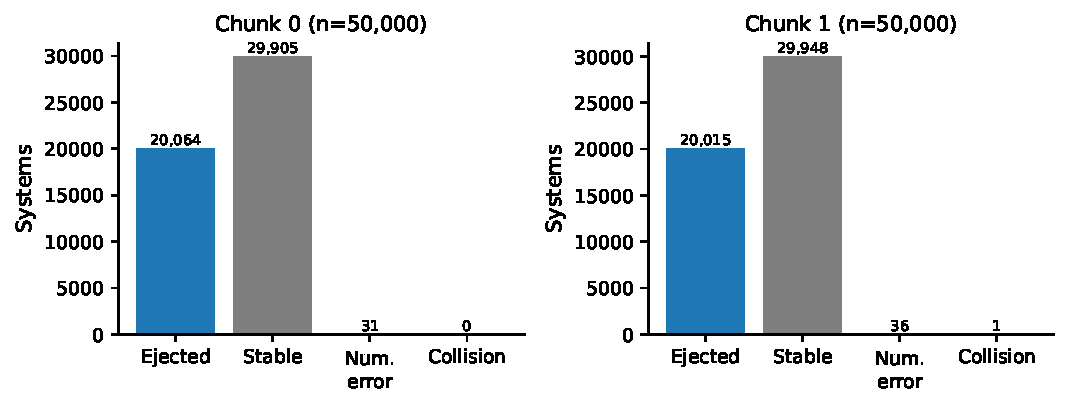
\includegraphics[width=\columnwidth]{figures/fig_tail_ledger.pdf}
  \caption{Matched deep-tail outcome counts by reintegration chunk (50,000
  systems each, seed 42). Generated from committed provenance metadata.}
  \label{fig:tail_ledger}
\end{figure}

\subsection{Finite-time ejection}
\todo{Insert final index-72/73-neutralized horizon curves and PR-based comparison.}

\subsection{Feature ablations and generalization}
Label-shuffle controls return chance discrimination.
\todo{Insert ablation and blocked-split table with uncertainty.}

\subsection{Lead time at fixed false-alarm rate}
\todo{Report per-horizon FAR separately from cumulative system-level false-alert
probability, with lead-time distributions.}

\subsection{Escaper and encounter outcome classes}
\todo{Report stable/outer-eject/inner-eject and flyby/exchange/ionization
macro-F1 and class recall.}

\subsection{Time remaining and hazards}
\todo{Report remaining-time regression and landmark Cox model with effect sizes,
not only p-values.}

\subsection{Partial AUC and literature baseline}
\todo{Insert \S10 partial-AUC and \S12 Vynatheya-baseline results once the
artifacts are public and committed.}
